\documentclass[aspectratio=169]{beamer}
\usepackage{tikz}
\usepackage{graphicx}
\usepackage{listings}
\usepackage{xcolor}
\usepackage{hyperref}
\usepackage[spanish,es-noquoting]{babel}
\usepackage[round]{natbib}

\lstset{
  basicstyle=\ttfamily\small,
  keywordstyle=\color{blue},
  stringstyle=\color{red},
  commentstyle=\color{gray},
  showstringspaces=false
}

% Clean Theme Setup & Optimization
\usetheme{Warsaw}
\usecolortheme{default}
\usefonttheme{serif}

% Remove top headline bar and navigation clutter to maximize slide text space
\setbeamertemplate{headline}{}
\setbeamertemplate{navigation symbols}{}

% Slim, clean footline bar
\setbeamertemplate{footline}{
  \leavevmode%
  \hbox{%
    \begin{beamercolorbox}[wd=.333333\paperwidth,ht=2.25ex,dp=1ex,left]{author in head/foot}%
      \hspace*{2ex}\insertshortauthor
    \end{beamercolorbox}%
    \begin{beamercolorbox}[wd=.333333\paperwidth,ht=2.25ex,dp=1ex,center]{title in head/foot}%
      \insertshorttitle
    \end{beamercolorbox}%
    \begin{beamercolorbox}[wd=.333333\paperwidth,ht=2.25ex,dp=1ex,right]{date in head/foot}%
      \insertframenumber{} / \inserttotalframenumber\hspace*{2ex}
    \end{beamercolorbox}%
  }%
  \vskip0pt%
}

% Font size and list spacing optimizations to prevent text overflow
\setbeamertemplate{itemize/enumerate body begin}{\small}
\setbeamertemplate{itemize/enumerate subbody begin}{\footnotesize}
\setbeamertemplate{itemize/enumerate subsubbody begin}{\scriptsize}

\makeatletter
\g@addto@macro\itemize{%
  \setlength{\itemsep}{2pt}%
  \setlength{\parsep}{1pt}%
  \setlength{\topsep}{2pt}%
  \setlength{\partopsep}{0pt}%
}
\makeatother

\graphicspath{{../}{./}}
\setbeamertemplate{caption}[numbered]

% Title info
\title[ PromptLibrary Jurídica (Sesió]{ PromptLibrary Jurídica (Sesión 1)}
\subtitle{ Qué es y por qué es la herramienta que más tiempo te va a ahorrar}
\author{Ricardo Reyes-Jimenez}
\institute{Universidad de La Sabana}
\date{\today}


% Background image for title slide
\usebackgroundtemplate{
  \tikz\node[opacity=0.3]{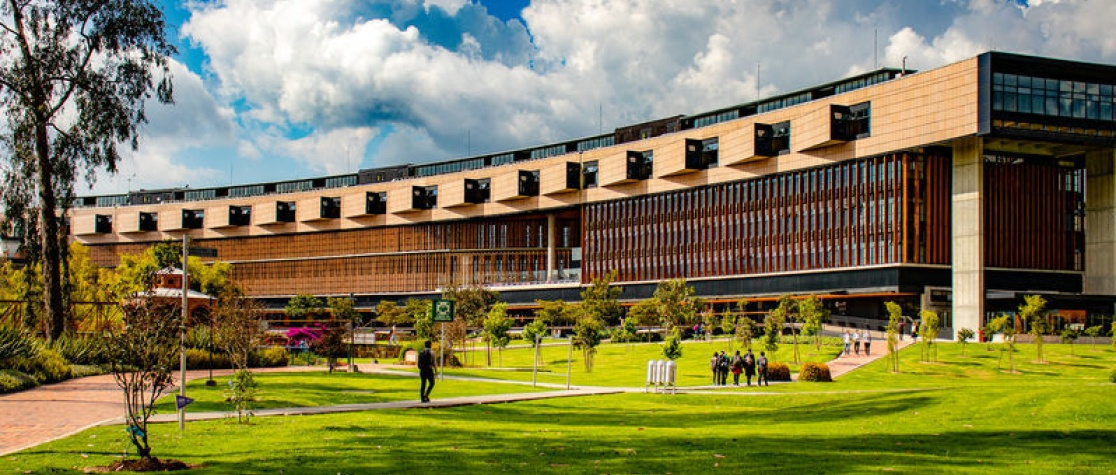
\includegraphics[width=\paperwidth,height=\paperheight]{Images/UniSabana.jpg}};
}


\begin{document}

% Title slide
\begin{frame}
  \titlepage
\end{frame}

% Reset background for normal slides
\usebackgroundtemplate{}


\begin{frame}[allowframebreaks,fragile]{Objetivos de la Sesión 1}

\begin{itemize}
  \item Entender qué es una PromptLibrary corporativa.
  \item Reconocer cómo soluciona los ``silos de conocimiento''.
  \item Aprender la anatomía de un ``Blueprint'' o plantilla reutilizable.
  \item Diseñar colaborativamente nuestros primeros prompts prácticos según nuestro rol (Litigio, Asesoría, Sector Público).
  \item Ejecutar y guardar nuestros primeros Blueprints en vivo.
\end{itemize}
\end{frame}

\begin{frame}[allowframebreaks,fragile]{La cruda realidad del trabajo manual}

\begin{itemize}
  \item Cada día, decenas de abogados en una firma realizan las mismas tareas: revisar cláusulas de indemnidad, resumir contestaciones de demanda, buscar jurisprudencia.
  \item \textbf{El costo:} Horas repetitivas que el cliente ya no quiere pagar.
  \item \textbf{El riesgo:} Errores humanos por fatiga en tareas mecánicas.
\end{itemize}
\end{frame}

\begin{frame}[allowframebreaks,fragile]{¿Qué es una PromptLibrary?}

\begin{itemize}
  \item \textbf{Definición:} Un repositorio centralizado, probado, documentado y categorizado de instrucciones (prompts) listas para usar por cualquier miembro del equipo.
  \item \textbf{Analogía Legal:} Es el equivalente al ``banco de modelos y minutas'' de la firma, pero para comunicarse con la Inteligencia Artificial.
\end{itemize}
\end{frame}

\begin{frame}[allowframebreaks,fragile]{El Problema: ``Ceguera del Prompt''}

\begin{itemize}
  \item Un asociado junior gasta 40 minutos experimentando hasta lograr que ChatGPT o Gemini genere un resumen perfecto de un expediente de 500 páginas.
  \item Logra su objetivo, cierra la pestaña y vuelve al trabajo.
  \item \textbf{Resultado:} Ese conocimiento (el prompt perfecto) se evaporó. Mañana, otro abogado empezará desde cero.
\end{itemize}
\end{frame}

\begin{frame}[allowframebreaks,fragile]{La Solución: Escalar el Conocimiento}

\begin{itemize}
  \item Si el asociado documenta ese prompt exitoso en la PromptLibrary...
  \item Los otros 50 abogados de la firma lo usarán mañana, reduciendo los 40 minutos de ensayo y error a 10 segundos.
  \item \textbf{El verdadero ROI de la IA no está en el uso individual, sino en el uso institucional.}
\end{itemize}
\end{frame}

\begin{frame}[allowframebreaks,fragile]{El Concepto de ``Blueprint'' (Plantilla)}

\begin{itemize}
  \item Un \textit{Blueprint} es un prompt parametrizado. No es un texto estático, sino un esqueleto o fórmula que permite sustituir variables.
  \item \textbf{Ejemplo Estático (Malo):} \textit{``Resume este contrato de arrendamiento de la calle 45.''}
  \item \textbf{Ejemplo Blueprint (Bueno):} \textit{``Actúa como abogado senior. Resume el siguiente [TIPO DE CONTRATO] enfocándote en [PUNTOS CLAVE A BUSCAR]. Contrato: [TEXTO]''}
\end{itemize}
\end{frame}

\begin{frame}[allowframebreaks,fragile]{Anatomía de un Prompt Reutilizable}

Todo buen \textit{Blueprint} en su biblioteca debe tener al menos 4 elementos documentados:
\begin{itemize}
  \item \textbf{Nombre y Rol:} Ej. \textit{Analista de Due Diligence M\&A}.
  \item \textbf{Contexto Base:} La instrucción inmutable (instrucciones de tono y formato).
  \item \textbf{Variables (Corchetes):} Los espacios que el usuario final debe rellenar.
  \item \textbf{Restricciones:} Lo que la IA \textit{nunca} debe hacer en este caso.
\end{itemize}
\end{frame}

\begin{frame}[allowframebreaks,fragile]{Variables Clave (El poder de los corchetes)}

El secreto de la PromptLibrary es usar corchetes \texttt{[ ]} para guiar al abogado usuario:
\begin{itemize}
  \item \texttt{[TIPO DE DOCUMENTO]}
  \item \texttt{[JURISDICCIÓN]}
  \item \texttt{[ROL DEL CLIENTE: Arrendador/Arrendatario]}
  \item \texttt{[TEXTO DEL EXPEDIENTE A PEGAR]}
\end{itemize}
\end{frame}

\begin{frame}[allowframebreaks,fragile]{Diferenciando por Rol: Litigio}

\textbf{Casos de uso para Blueprints en Litigio:}
\begin{itemize}
  \item \textbf{Extracción de Hechos:} Extraer cronologías exactas a partir de correos cruzados.
  \item \textbf{Identificación de Inconsistencias:} Cruzar el interrogatorio del testigo con su declaración juramentada previa.
  \item \textbf{Borradores:} Esquematizar la estructura de una contestación de demanda basándose en los hechos alegados.
\end{itemize}
\end{frame}

\begin{frame}[allowframebreaks,fragile]{Diferenciando por Rol: Asesoría Corporativa}

\textbf{Casos de uso para Blueprints en Asesoría (Corporate/M\&A):}
\begin{itemize}
  \item \textbf{Red-Flagging:} Búsqueda rápida de cláusulas de cambio de control, exclusividad o penalidades en un \textit{Data Room}.
  \item \textbf{Resúmenes Ejecutivos:} Transformar un documento técnico de 40 páginas en un memo de 2 páginas para la junta directiva.
  \item \textbf{Traducción Legal:} Adaptar un contrato con jerga de Common Law a conceptos del derecho civil local.
\end{itemize}
\end{frame}

\begin{frame}[allowframebreaks,fragile]{Diferenciando por Rol: Sector Público}

\textbf{Casos de uso para Blueprints en Sector Público:}
\begin{itemize}
  \item \textbf{Derechos de Petición:} Analizar las pretensiones del ciudadano y compararlas con las plantillas de respuesta de la entidad.
  \item \textbf{Licitaciones:} Verificación cruzada (checklist) de cumplimiento de requisitos habilitantes en propuestas de miles de páginas.
  \item \textbf{Proyección de Fallos:} Estructuración de los antecedentes y consideraciones iniciales.
\end{itemize}
\end{frame}

\begin{frame}[allowframebreaks,fragile]{Herramientas para empezar HOY}

\textbf{No necesitas software de $10,000 USD para arrancar (Fase 1)}
\begin{itemize}
  \item La fricción mata la innovación. Si el sistema es complejo, nadie lo usará.
  \item \textbf{Recomendación:} Empezar hoy mismo con un documento colaborativo (Word Online, Excel, Google Sheets o Notion).
  \item Lo importante no es la plataforma, es la disciplina de documentar el \textit{Blueprint}.
\end{itemize}
\end{frame}

\begin{frame}[allowframebreaks,fragile]{Demo: Así se ve una Versión 1.0}

\textit{(El Mentor muestra un Excel en pantalla)}
\begin{itemize}
  \item \textbf{Columna A:} Nombre del Prompt.
  \item \textbf{Columna B:} Caso de uso.
  \item \textbf{Columna C:} Blueprint (con variables en negrita).
  \item \textbf{Columna D:} Autor / Fecha.
  \item \textbf{Columna E:} Eficacia estimada (Del 1 al 5).
\end{itemize}
\end{frame}

\begin{frame}[allowframebreaks,fragile]{Taller Práctico (Fase 1): Identificación}

\textbf{Trabajo en grupos por roles (15 minutos)}
\begin{itemize}
  \item Reúnanse con colegas de áreas de práctica similares.
  \item Identifiquen \textbf{UNA} tarea repetitiva, aburrida y de bajo valor estratégico que realicen todas las semanas.
  \item Definan el objetivo exacto que quieren que la IA logre.
\end{itemize}
\end{frame}

\begin{frame}[allowframebreaks,fragile]{Taller Práctico (Fase 2): Redacción del Blueprint}

\textbf{Redacción (20 minutos)}
\begin{itemize}
  \item Utilizando los frameworks del Módulo 2 (CARE/TAM), escriban el \textit{Blueprint} maestro.
  \item Asegúrense de usar corchetes \texttt{[ ]} para las partes que cambian caso a caso.
  \item Incluyan restricciones claras (ej. ``Usa viñetas, no uses lenguaje poético, omite saludos'').
\end{itemize}
\end{frame}

\begin{frame}[allowframebreaks,fragile]{Taller Práctico (Fase 3): Pruebas de Fuego}

\textbf{Ejecución en Vivo (20 minutos)}
\begin{itemize}
  \item Abran su asistente de IA (ChatGPT, Gemini, Claude).
  \item Copien su \textit{Blueprint}, llenen los corchetes con un caso real (anonimizado) y ejecútenlo.
  \item ¿El resultado fue perfecto a la primera? (Spoiler: Casi nunca lo es). Anoten qué falló.
\end{itemize}
\end{frame}

\begin{frame}[allowframebreaks,fragile]{Cierre de Sesión 1}

\begin{itemize}
  \item Hoy pasamos del conocimiento tácito al conocimiento documentado.
  \item Ya tienen en sus manos su primer activo institucional: un Blueprint funcional.
  \item \textbf{Para la próxima sesión:} Veremos cómo refinar estos prompts que fallaron, cómo compartirlos y cómo escalar este Excel a un sistema institucional a prueba del tiempo. ¡Guarden sus archivos!
\end{itemize}
\end{frame}




\end{document}